\documentclass[conference,twocolumn]{IEEEtran}
\IEEEoverridecommandlockouts

\usepackage{cite}
\usepackage{amsmath,amssymb,amsfonts}
\usepackage{algorithmic}
\usepackage{graphicx}
\usepackage{textcomp}
\usepackage{xcolor}
\usepackage{booktabs}
\usepackage{multirow}
\usepackage{array}
\usepackage{tabularx}
\usepackage{float}
\usepackage[pdfa]{hyperref}
\usepackage{subcaption}
\usepackage{balance}
\usepackage{stfloats}
\usepackage{placeins}
\setcounter{dbltopnumber}{2}
\renewcommand{\dbltopfraction}{0.95}
\renewcommand{\dblfloatpagefraction}{0.85}
\usepackage[font=small,labelfont=bf,skip=4pt]{caption}
\usepackage[margin=0.7in]{geometry}

% Tighter spacing
\setlength{\textfloatsep}{6pt}
\setlength{\floatsep}{6pt}
\setlength{\intextsep}{6pt}
\captionsetup{justification=raggedright,singlelinecheck=false}

\graphicspath{{img/}{figures/}}

\def\BibTeX{{\rm B\kern-.05em{\sc i\kern-.025em b}\kern-.08em
    T\kern-.1667em\lower.7ex\hbox{E}\kern-.125emX}}

% Define model name macro for consistent usage
\newcommand{\modelname}{MicroBiConvLSTM}
\newcommand{\modelnameplain}{MicroBiConvLSTM}

\begin{document}

\title{MicroBiConvLSTM: A Lightweight Efficient Model for Human Activity Recognition on Resource Constrained Devices}

\author{\IEEEauthorblockN{Group Number 14}
\IEEEauthorblockA{Mridankan Mandal, IIB2024017 \quad Aditya Pachauri, IIB2024001\\
Dhannu Ram Meena, IIB2024033 \quad Ankit Ekka, IIB2024012}
}

\maketitle

\begin{abstract}
Human Activity Recognition (HAR) on resource constrained wearables requires models that balance accuracy with strict memory and computation limits. Lightweight architectures such as TinierHAR with 34K parameters and TinyHAR with 55K parameters achieve strong accuracy. Their size can still limit deployment on small microcontrollers.

\modelname{} is a lightweight convolutional recurrent architecture with 11.4K parameters on average. It uses two stage convolutional feature extraction, 4$\times$ temporal pooling and one bidirectional LSTM layer. This design reduces parameters by 2.9$\times$ versus TinierHAR and 11.9$\times$ versus DeepConvLSTM while preserving linear $O(N)$ complexity.

Evaluation on eight HAR benchmarks shows competitive performance in the lightweight regime. \modelname{} reaches 93.41\% macro F1 on UCI-HAR, 94.46\% on SKODA assembly gestures and 88.98\% on Daphnet gait freeze detection. Ablation results show that bidirectionality helps episodic event detection while giving limited gains on periodic locomotion.
\end{abstract}

\section{Introduction}

Human Activity Recognition (HAR) from wearable inertial sensors supports health monitoring, fall detection and fitness tracking. These tasks often run on wearable devices with strict limits on memory, computation and battery use.

DeepConvLSTM \cite{ordonez2016deep} provides a strong convolutional recurrent baseline. In our benchmark implementation, it averages 136K parameters and 15.5M MACs. TinyHAR \cite{zhou2022tinyhar} uses cross channel attention and averages 55K parameters in our implementation. TinierHAR \cite{bian2025tinierhar} uses depthwise separable convolutions and bidirectional GRUs and averages 34K parameters. These models improve efficiency, though a smaller model is still useful for devices with limited SRAM.

Microcontrollers also reserve memory for system software, sensor drivers and communication. The available model budget can therefore be much smaller than the total SRAM. This gap motivates a compact architecture that preserves temporal modeling capacity.

We introduce \modelname{}, designed to maximize information density within a constrained parameter budget. Our contributions are:
\begin{itemize}
    \item An 11.4K parameter architecture on average. A two stage convolutional stem, 4$\times$ temporal pooling and one bidirectional LSTM give a 2.9$\times$ parameter reduction versus TinierHAR while keeping $O(N)$ complexity.
    \item Evaluation across eight HAR benchmarks. The results define the accuracy and efficiency tradeoff across datasets with different sensor counts and class distributions.
    \item Ablation studies that isolate task dependent effects. Bidirectionality helps episodic events while it is optional for periodic activities.
\end{itemize}

Figure~\ref{fig:architecture} shows the architecture. The design uses 11.4K parameters on average with strict $O(N)$ complexity. It targets memory constrained environments.

\begin{figure*}[t]
    \centering
    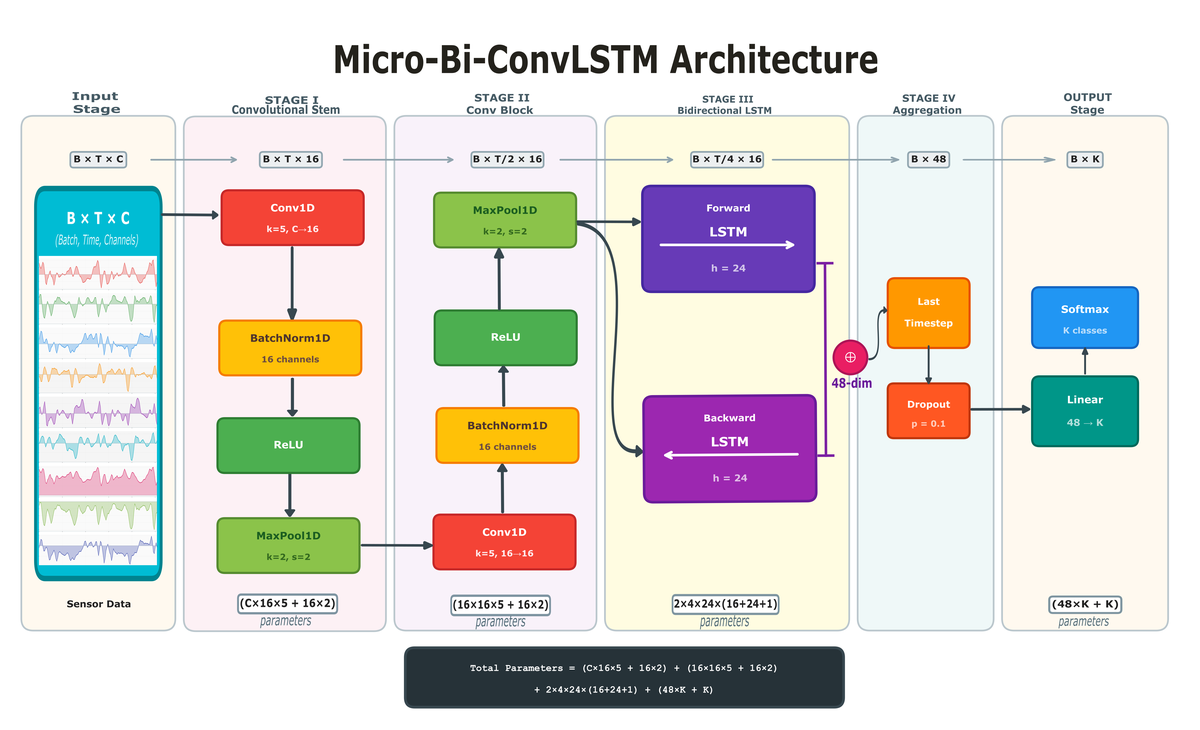
\includegraphics[width=0.85\textwidth]{img/LightDeepConvLSTM_Architecture.png}
    \caption{\modelname{} architecture overview. Input sensor signals ($C$ channels $\times$ $T$ timesteps) pass through two convolutional blocks with batch normalization, ReLU activation and 2$\times$ max pooling in each block. This gives 4$\times$ temporal compression. A single bidirectional LSTM with hidden dimension 24 processes the compressed sequence. The final timestep representation feeds the classification head. Parameter count varies with input channels and output classes.}
    \label{fig:architecture}
\end{figure*}

\section{Related Work}\vspace{-1mm}

DeepConvLSTM \cite{ordonez2016deep} combines convolutional feature extraction with recurrent temporal modeling. TinyHAR \cite{zhou2022tinyhar} adds cross channel attention. TinierHAR \cite{bian2025tinierhar} uses depthwise separable convolutions and bidirectional GRUs. These three models are the direct baselines for our evaluation.

Knowledge distillation trains a compact student from softened class probabilities produced by a larger frozen teacher while leaving the student inference architecture unchanged \cite{hinton2015distilling}. Teacher assistant distillation inserts an intermediate model when the capacity gap between teacher and student is large \cite{mirzadeh2020improved}. We evaluate both routes with \modelname{} as the student.

Table~\ref{tab:architecture_comparison} compares the main architecture choices. \modelname{} uses 4$\times$ temporal pooling and standard convolutions that preserve cross channel information. The sequence cost remains $O(N)$.

\begin{table}[t]
\centering
\caption{Architectural Comparison of HAR Models}
\label{tab:architecture_comparison}
\resizebox{\columnwidth}{!}{%
\begin{tabular}{@{}lccccc@{}}
\toprule
\textbf{Model} & \textbf{Conv Type} & \textbf{Temporal} & \textbf{Attention} & \textbf{Params $\downarrow$} & \textbf{Complexity} \\
\midrule
DeepConvLSTM & Standard & 2$\times$LSTM & No & 136K & $O(N)$ \\
TinyHAR & Standard & LSTM+Attn & Yes & 55K & $O(N^2)$ \\
TinierHAR & Depthwise & BiGRU+Attn & Yes & 34K & $O(N^2)$ \\
\modelnameplain{} & Standard & BiLSTM & No & \textbf{11.4K} & $O(N)$ \\
\bottomrule
\end{tabular}%
}\vspace{-2mm}
\end{table}

\section{Methodology}\vspace{-1mm}

\modelname{} (Figure~\ref{fig:architecture}) has a two stage convolutional stem followed by one bidirectional LSTM. Five principles guide the design. First, 4$\times$ temporal pooling reduces the LSTM sequence length. Second, standard convolutions preserve cross channel information in low dimensional sensor data. Third, one BiLSTM with $H=24$ avoids redundant stacking. Fourth, bidirectional processing captures temporal asymmetry in episodic events. Fifth, $O(N)$ complexity gives predictable inference cost.

\textbf{Convolutional Stages}: Input $\mathbf{X} \in \mathbb{R}^{B \times T \times C}$ passes through two convolutional blocks with $F=16$ filters and kernel size $K=5$. Each block uses batch normalization, ReLU and 2$\times$ max pooling. The output has $T/4$ timesteps and a 9 timestep receptive field.

\textbf{Bidirectional LSTM}: Compressed features pass through a single layer BiLSTM with hidden dimension $H=24$. Forward and backward states form a 48 dimensional representation. Last timestep aggregation ($\mathbf{h}_{\text{agg}} = \mathbf{H}[:, -1, :]$) avoids attention overhead while retaining sequence context.

\textbf{Classification}: Dropout regularization followed by linear classifier with softmax output.

\textbf{Complexity}: Parameters range from 10K to 32K across datasets (Table~\ref{tab:efficiency}). The BiLSTM accounts for about 75\% of the parameters. MACs scale linearly from 245K to 1.14M. This is a 32 to 42$\times$ reduction compared with DeepConvLSTM.

\textbf{Knowledge Distillation}: Let $z_t$ and $z_s$ denote teacher and student logits. We freeze the teacher and minimize
\begin{equation}
\begin{aligned}
\mathcal{L} &= (1-\alpha)\mathcal{L}_{\mathrm{CE}}+\alpha T^2D_{\mathrm{KL}}\!\left(p_t^T\,\|\,p_s^T\right),\\
p^T &= \operatorname{softmax}(z/T),
\end{aligned}
\end{equation}
where $\mathcal{L}_{\mathrm{CE}}$ is class weighted cross entropy. Direct distillation transfers softened teacher outputs to \modelname{} \cite{hinton2015distilling}. The assistant route first distills the teacher into an intermediate model, then freezes that model and distills it into \modelname{} \cite{mirzadeh2020improved}. Both routes preserve the student architecture and inference cost.

\section{Experimental Setup}\vspace{-1mm}

\textbf{Datasets}: Eight HAR benchmarks appear in Table~\ref{tab:datasets}. They cover smartphone IMU data, body worn IMU data, fall detection and industrial gestures. The counts in Table~\ref{tab:datasets} describe the dataset versions and processed inputs used in our experiments.

\textbf{Preprocessing}: Noisy datasets use Butterworth low pass filtering at 10~Hz for PAMAP2, 5~Hz for SKODA and 12~Hz for Daphnet. The pipeline applies channel wise standardization, sliding windows with 50\% overlap and subject wise cross validation for datasets with multiple subjects.

\textbf{Training}: Training uses AdamW with cosine annealing for at most 200 epochs and early stopping patience of ten. Fifty TPE trials search the learning rate from $10^{-4}$ to $10^{-2}$, weight decay from $10^{-5}$ to $5{\times}10^{-2}$ and dropout from 0.0 to 0.5. Inverse frequency weighting handles class imbalance. Results report the mean macro F1 score and standard deviation over five runs from a master seed.

\textbf{Baselines}: We implement DeepConvLSTM \cite{ordonez2016deep}, TinyHAR \cite{zhou2022tinyhar} and TinierHAR \cite{bian2025tinierhar} following their cited designs. Across datasets, our implementations average 136K, 55K and 34K parameters, respectively. All neural models use the same hyperparameter search and training protocol.

\textbf{Knowledge Distillation}: We evaluate on PAMAP2, WISDM, UniMiB, UCI-HAR and SKODA datasets. The teacher and assistant pairs are TinierHAR and TinyHAR on PAMAP2, TinierHAR and DeepConvLSTM on WISDM, DeepConvLSTM and TinierHAR on UniMiB and TinyHAR and TinierHAR on UCI-HAR and SKODA. Temperature is $T=4$ and the soft loss weight is $\alpha=0.5$. Master seed 17 generates five random seeds. Every route uses the same preprocessing, partitions and training schedule as the corresponding non distilled student. The checkpoint with the highest held out macro F1 score is retained.

\textbf{Classical Baselines}: We evaluate multinomial logistic regression, a RBF SVM and XGBoost \cite{chen2016xgboost}. Each sensor channel gives 21 descriptors for location, dispersion, quantiles, energy, moments, first differences and frequency content. This produces $21C$ features for $C$ channels. Nonfinite values use deterministic replacement. Logistic regression and SVM standardize features using training data. The SVM also uses 64 component PCA fit on training data. XGBoost uses unscaled features and balanced sample weights. Logistic regression uses $C=1$ with the lbfgs solver. The SVM uses $C=10$ with gamma set to scale. XGBoost uses 300 depth six trees, learning rate 0.05 and row and column subsampling of 0.8. All training windows are retained. Master seed 17 is used to generate five random seeds. The baselines use the same dataset partitions. Learned preprocessing uses training data only. The held out split is used once for final evaluation.

\begin{table}[t]
\centering
\caption{Processed Dataset Configuration}
\label{tab:datasets}
\resizebox{\columnwidth}{!}{%
\begin{tabular}{@{}lccccccc@{}}
\toprule
\textbf{Dataset} & \textbf{Type} & \textbf{Subjects} & \textbf{Classes} & \textbf{Channels} & \textbf{Frequency} & \textbf{Window} \\
\midrule
UCI-HAR \cite{anguita2013public} & Phone & 30 & 6 & 9 & 50 Hz & 128 \\
MotionSense \cite{malekzadeh2019mobile} & Phone & 24 & 6 & 6 & 50 Hz & 128 \\
WISDM \cite{kwapisz2011activity} & Phone & 36 & 6 & 3 & 20 Hz & 128 \\
PAMAP2 \cite{reiss2012introducing} & Body IMU & 9 & 12 & 19 & 100 Hz & 128 \\
Opportunity \cite{chavarriaga2013opportunity} & Body IMU & 4 & 5 & 79 & 30 Hz & 128 \\
UniMiB \cite{micucci2017unimib} & Phone & 30 & 9 & 3 & 50 Hz & 128 \\
SKODA \cite{stiefmeier2008wearable} & Glove IMU & 1 & 11 & 30 & 98 Hz & 98 \\
Daphnet \cite{bachlin2010wearable} & Body IMU & 10 & 2 & 9 & 64 Hz & 64 \\
\bottomrule
\end{tabular}%
}
\end{table}
\vspace{-2mm}

\section{Results}\vspace{-1mm}

\subsection{Predictive Performance}

Table~\ref{tab:f1_comparison} presents F1 scores across all benchmarks. With 2.9$\times$ fewer parameters than TinierHAR, \modelname{} has a 3.12\% gap on UCI-HAR and a 1.02\% gap on MotionSense. It reaches 88.98\% on Daphnet, close to TinierHAR at 89.84\% and above TinyHAR at 86.42\%. PAMAP2 has the largest gap at 13.3\%. Figure~\ref{fig:benchmark_comparison} shows the performance distributions.

\begin{figure*}[!t]
    \centering
    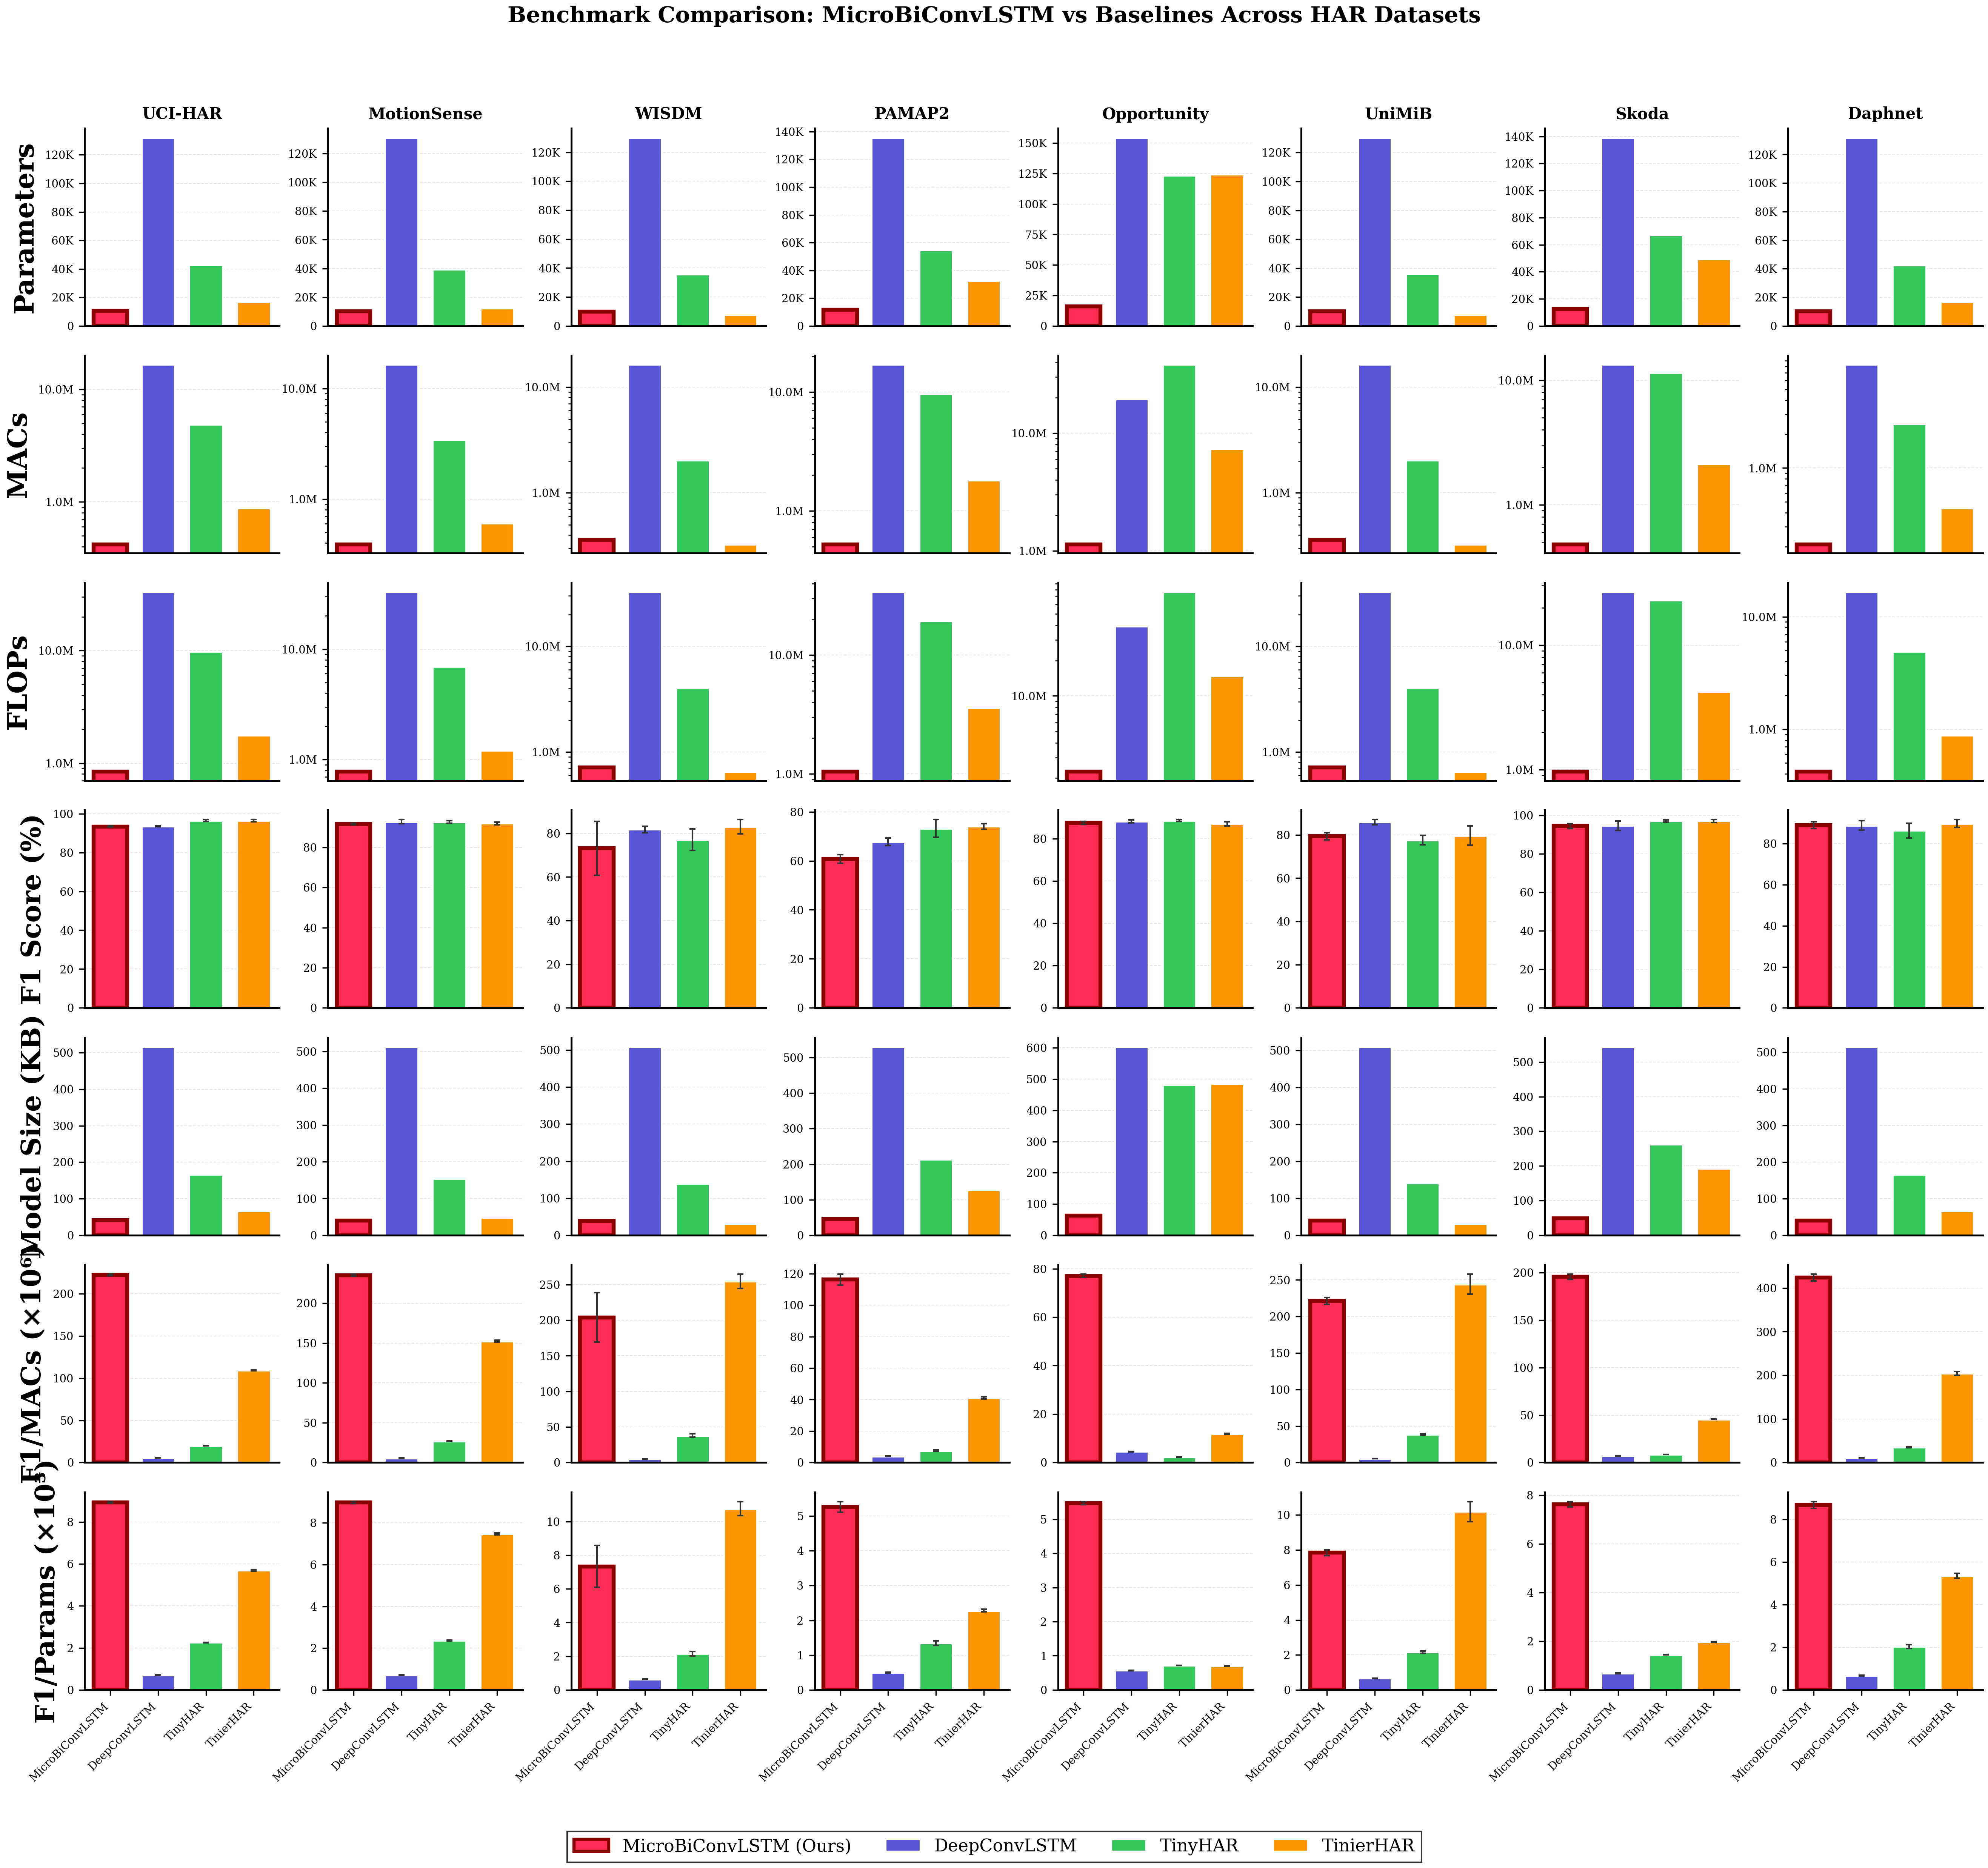
\includegraphics[width=0.82\textwidth]{img/benchmark_comparison_grid.png}
    \caption{Cross dataset comparison of parameter count, MACs, FLOPs, macro F1, model size, F1 per MAC and F1 per parameter. Macro F1 error bars show standard deviations across five random seeds.}
    \label{fig:benchmark_comparison}
\end{figure*}

\textbf{Class Imbalance Sensitivity}: PAMAP2 has a 13.3\% F1 score gap. Rare activities form less than 10\% of its samples. This makes macro F1 difficult for a low capacity model. Opportunity gives 87.58\% for \modelname{} and 87.09\% for TinierHAR despite its 79 channels. This result suggests that class distribution can matter more than sensor dimension.

\begin{table}[t]
\centering
\caption{F1 Score Comparison (Macro \%)}
\label{tab:f1_comparison}
\resizebox{\columnwidth}{!}{%
\begin{tabular}{@{}lcccc@{}}
\toprule
\textbf{Dataset} & \textbf{\modelnameplain{} $\uparrow$} & \textbf{DeepConvLSTM $\uparrow$} & \textbf{TinyHAR $\uparrow$} & \textbf{TinierHAR $\uparrow$} \\
\midrule
UCI-HAR & 93.41$\pm$0.35 & 93.61$\pm$0.56 & 96.53$\pm$0.41 & 96.37$\pm$0.59 \\
MotionSense & 91.65$\pm$0.43 & 91.64$\pm$0.75 & 92.67$\pm$0.67 & 91.99$\pm$0.60 \\
WISDM & 73.17$\pm$12.4 & 81.25$\pm$2.55 & 77.09$\pm$4.95 & 83.06$\pm$3.24 \\
PAMAP2 & 60.75$\pm$1.76 & 66.20$\pm$2.72 & 73.22$\pm$3.58 & 74.07$\pm$1.16 \\
Opportunity & 87.58$\pm$0.73 & 87.21$\pm$0.63 & 88.69$\pm$0.38 & 87.09$\pm$0.90 \\
UniMiB & 79.43$\pm$1.66 & 84.12$\pm$2.23 & 77.61$\pm$2.23 & 79.67$\pm$4.45 \\
SKODA & 94.46$\pm$1.31 & 95.25$\pm$1.03 & 97.01$\pm$0.53 & 96.99$\pm$0.76 \\
Daphnet & 88.98$\pm$1.64 & 88.19$\pm$1.89 & 86.42$\pm$3.64 & 89.84$\pm$1.90 \\
\midrule
\textbf{Average} & 83.68 & 85.93 & 86.16 & \textbf{87.39} \\
\bottomrule
\end{tabular}%
}
\end{table}

\subsection{Classical Baselines}

Table~\ref{tab:classical_f1} reports five seed macro F1 scores for the classical baselines. \modelname{} has the highest cross dataset average at 83.68\%. The RBF SVM reaches 82.02\%. This is 1.66 points lower. XGBoost has the highest score on MotionSense, WISDM, Opportunity and SKODA. The RBF SVM has the highest score on PAMAP2. \modelname{} has the highest score on UCI-HAR, UniMiB and Daphnet.

\begin{table}[t]
\centering
\caption{Macro F1 Scores for \modelnameplain{} and Classical Baselines (\%)}
\label{tab:classical_f1}
\resizebox{\columnwidth}{!}{%
\begin{tabular}{@{}lcccc@{}}
\toprule
\textbf{Dataset} & \textbf{\modelnameplain{} $\uparrow$} & \textbf{Logistic $\uparrow$} & \textbf{RBF SVM $\uparrow$} & \textbf{XGBoost $\uparrow$} \\
\midrule
UCI-HAR & 93.41$\pm$0.35 & 92.70$\pm$0.00 & 92.71$\pm$0.04 & 92.81$\pm$0.09 \\
MotionSense & 91.65$\pm$0.43 & 89.43$\pm$0.00 & 90.47$\pm$0.02 & 93.51$\pm$0.14 \\
WISDM & 73.17$\pm$12.40 & 75.12$\pm$0.00 & 80.11$\pm$0.00 & 84.61$\pm$0.31 \\
PAMAP2 & 60.75$\pm$1.76 & 59.20$\pm$0.00 & 77.23$\pm$0.38 & 56.49$\pm$0.58 \\
Opportunity & 87.58$\pm$0.73 & 84.92$\pm$0.00 & 88.29$\pm$0.12 & 89.26$\pm$0.19 \\
UniMiB & 79.43$\pm$1.66 & 62.16$\pm$0.00 & 67.55$\pm$0.00 & 65.27$\pm$0.93 \\
SKODA & 94.46$\pm$1.31 & 96.01$\pm$0.00 & 96.92$\pm$0.09 & 99.53$\pm$0.10 \\
Daphnet & 88.98$\pm$1.64 & 63.01$\pm$0.00 & 62.90$\pm$0.38 & 68.83$\pm$0.76 \\
\midrule
\textbf{Average} & 83.68 & 77.82 & 82.02 & 81.29 \\
\bottomrule
\end{tabular}%
}
\end{table}

Table~\ref{tab:classical_efficiency} compares macro F1, compact state size and CPU cycle efficiency across model families. The benchmark processes one complete raw window on one pinned CPU thread. All measurements average five seeds across PAMAP2, WISDM, UniMiB, UCI-HAR and SKODA. Each classical path includes feature extraction, FFT operations, scaling, PCA when required and prediction. State size uses a compact FP32 equivalent inference representation instead of a serialized framework container. The measurements show that \modelname{} has the highest macro F1 and the best cycle efficiency. Logistic regression has the smallest state and the best storage efficiency.

\begin{table}[t]
\centering
\caption{Raw Window Inference Efficiency}
\label{tab:classical_efficiency}
\resizebox{\columnwidth}{!}{%
\begin{tabular}{@{}lccccc@{}}
\toprule
\textbf{Model} & \textbf{Macro F1 (\%) $\uparrow$} & \textbf{State (KiB) $\downarrow$} & \textbf{Mcycles/window $\downarrow$} & \textbf{F1/KiB $\uparrow$} & \textbf{F1/Mcycle $\uparrow$} \\
\midrule
\textbf{\modelnameplain{}} & \textbf{82.96} & 42.83 & \textbf{0.491} & 1.937 & \textbf{169.081} \\
Logistic Regression & 77.04 & \textbf{12.91} & 1.065 & \textbf{5.966} & 72.338 \\
PCA RBF SVM & 82.90 & 1,160.99 & 1.631 & 0.071 & 50.828 \\
XGBoost & 79.74 & 864.63 & 2.404 & 0.092 & 33.171 \\
\bottomrule
\end{tabular}%
}
\end{table}

\subsection{Knowledge Distillation}

Table~\ref{tab:kd_results} compares the non distilled student with direct teacher to student distillation and teacher assistant student distillation. Direct distillation gives the clearest gain on PAMAP2. Macro F1 increases by 2.71 points and all five paired runs improve. Direct distillation also gives smaller mean gains on UniMiB and SKODA. The assistant route gives small gains on UniMiB and UCI-HAR. The remaining comparisons show small or negative changes.

\begin{table}[H]
\centering
\caption{Knowledge Distillation Results (Macro F1 \%). Values are mean $\pm$ standard deviation over five seeds.}
\label{tab:kd_results}
\resizebox{\columnwidth}{!}{%
\begin{tabular}{@{}lccccc@{}}
\toprule
\textbf{Dataset} & \textbf{Base $\uparrow$} & \textbf{Direct KD $\uparrow$} & \textbf{$\Delta$ Direct $\uparrow$} & \textbf{Assistant KD $\uparrow$} & \textbf{$\Delta$ Assistant $\uparrow$} \\
\midrule
PAMAP2 & 65.02$\pm$2.10 & \textbf{67.73$\pm$3.33} & \textbf{+2.71} & 63.58$\pm$3.78 & $-$1.44 \\
WISDM & \textbf{80.87$\pm$2.71} & 79.89$\pm$1.29 & $-$0.98 & 80.82$\pm$2.43 & $-$0.05 \\
UniMiB & 79.23$\pm$5.80 & \textbf{80.56$\pm$2.79} & \textbf{+1.33} & 79.42$\pm$2.12 & +0.19 \\
UCI-HAR & 93.01$\pm$0.63 & 92.79$\pm$0.32 & $-$0.22 & \textbf{93.24$\pm$0.27} & \textbf{+0.23} \\
SKODA & 96.67$\pm$0.91 & \textbf{97.22$\pm$0.76} & \textbf{+0.56} & 96.40$\pm$0.95 & $-$0.27 \\
\bottomrule
\end{tabular}%
}
\end{table}

\begin{figure}[H]
    \centering
    \begin{subfigure}[b]{0.48\columnwidth}
        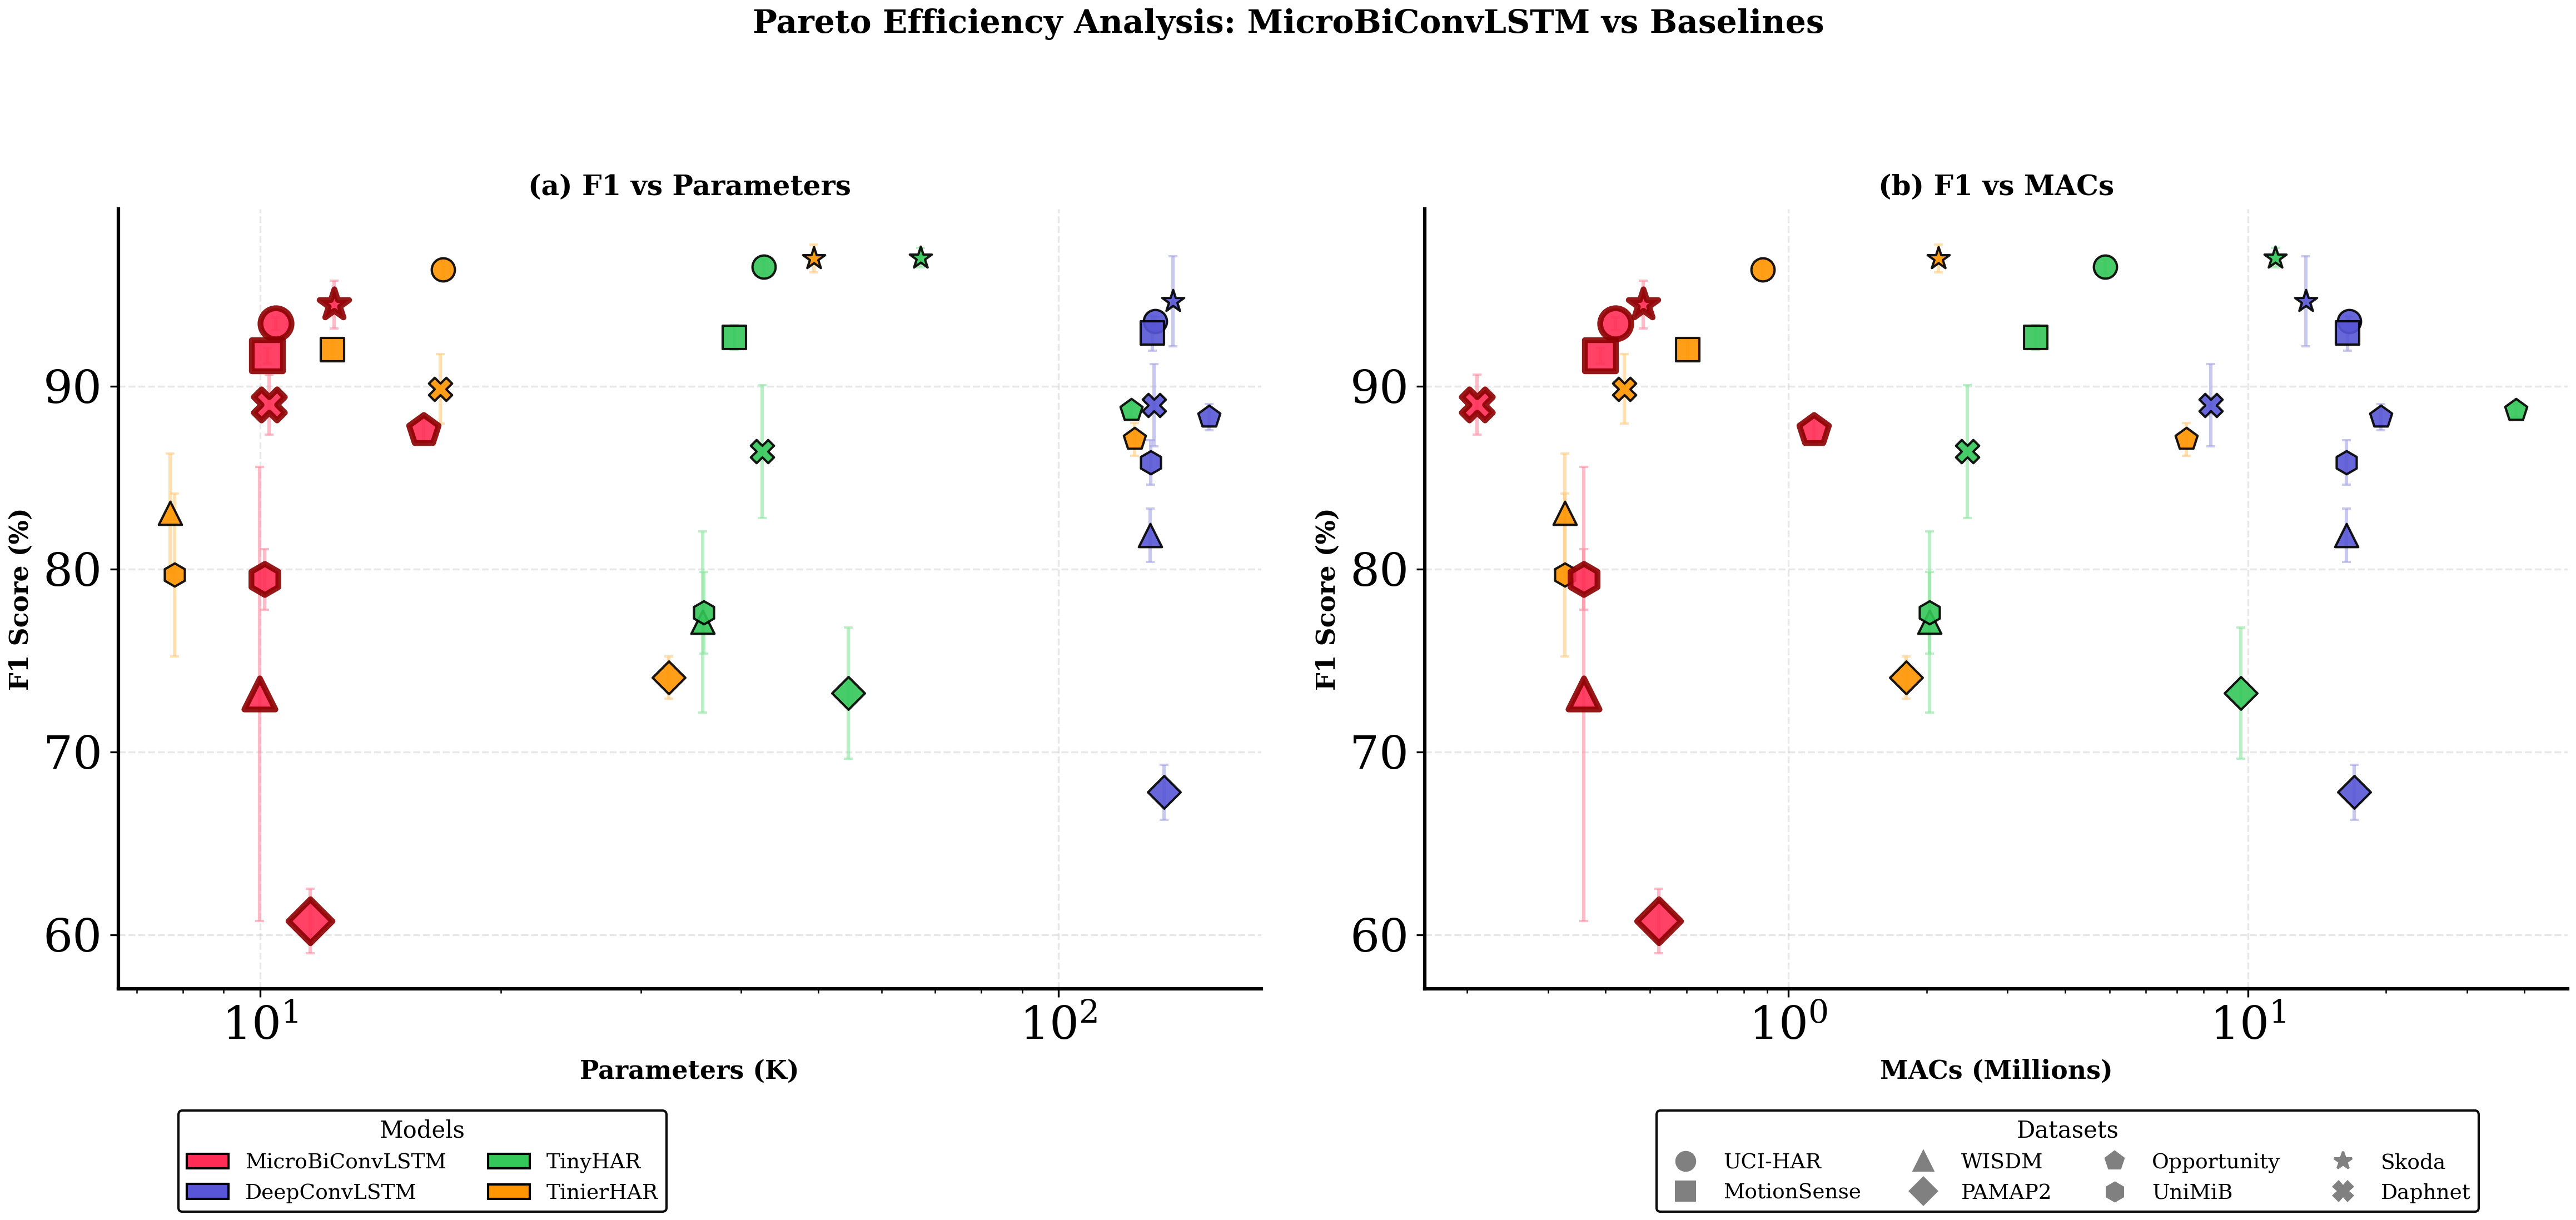
\includegraphics[width=\textwidth]{img/pareto_efficiency.png}
        \caption{Pareto frontier}
    \end{subfigure}
    \hfill
    \begin{subfigure}[b]{0.48\columnwidth}
        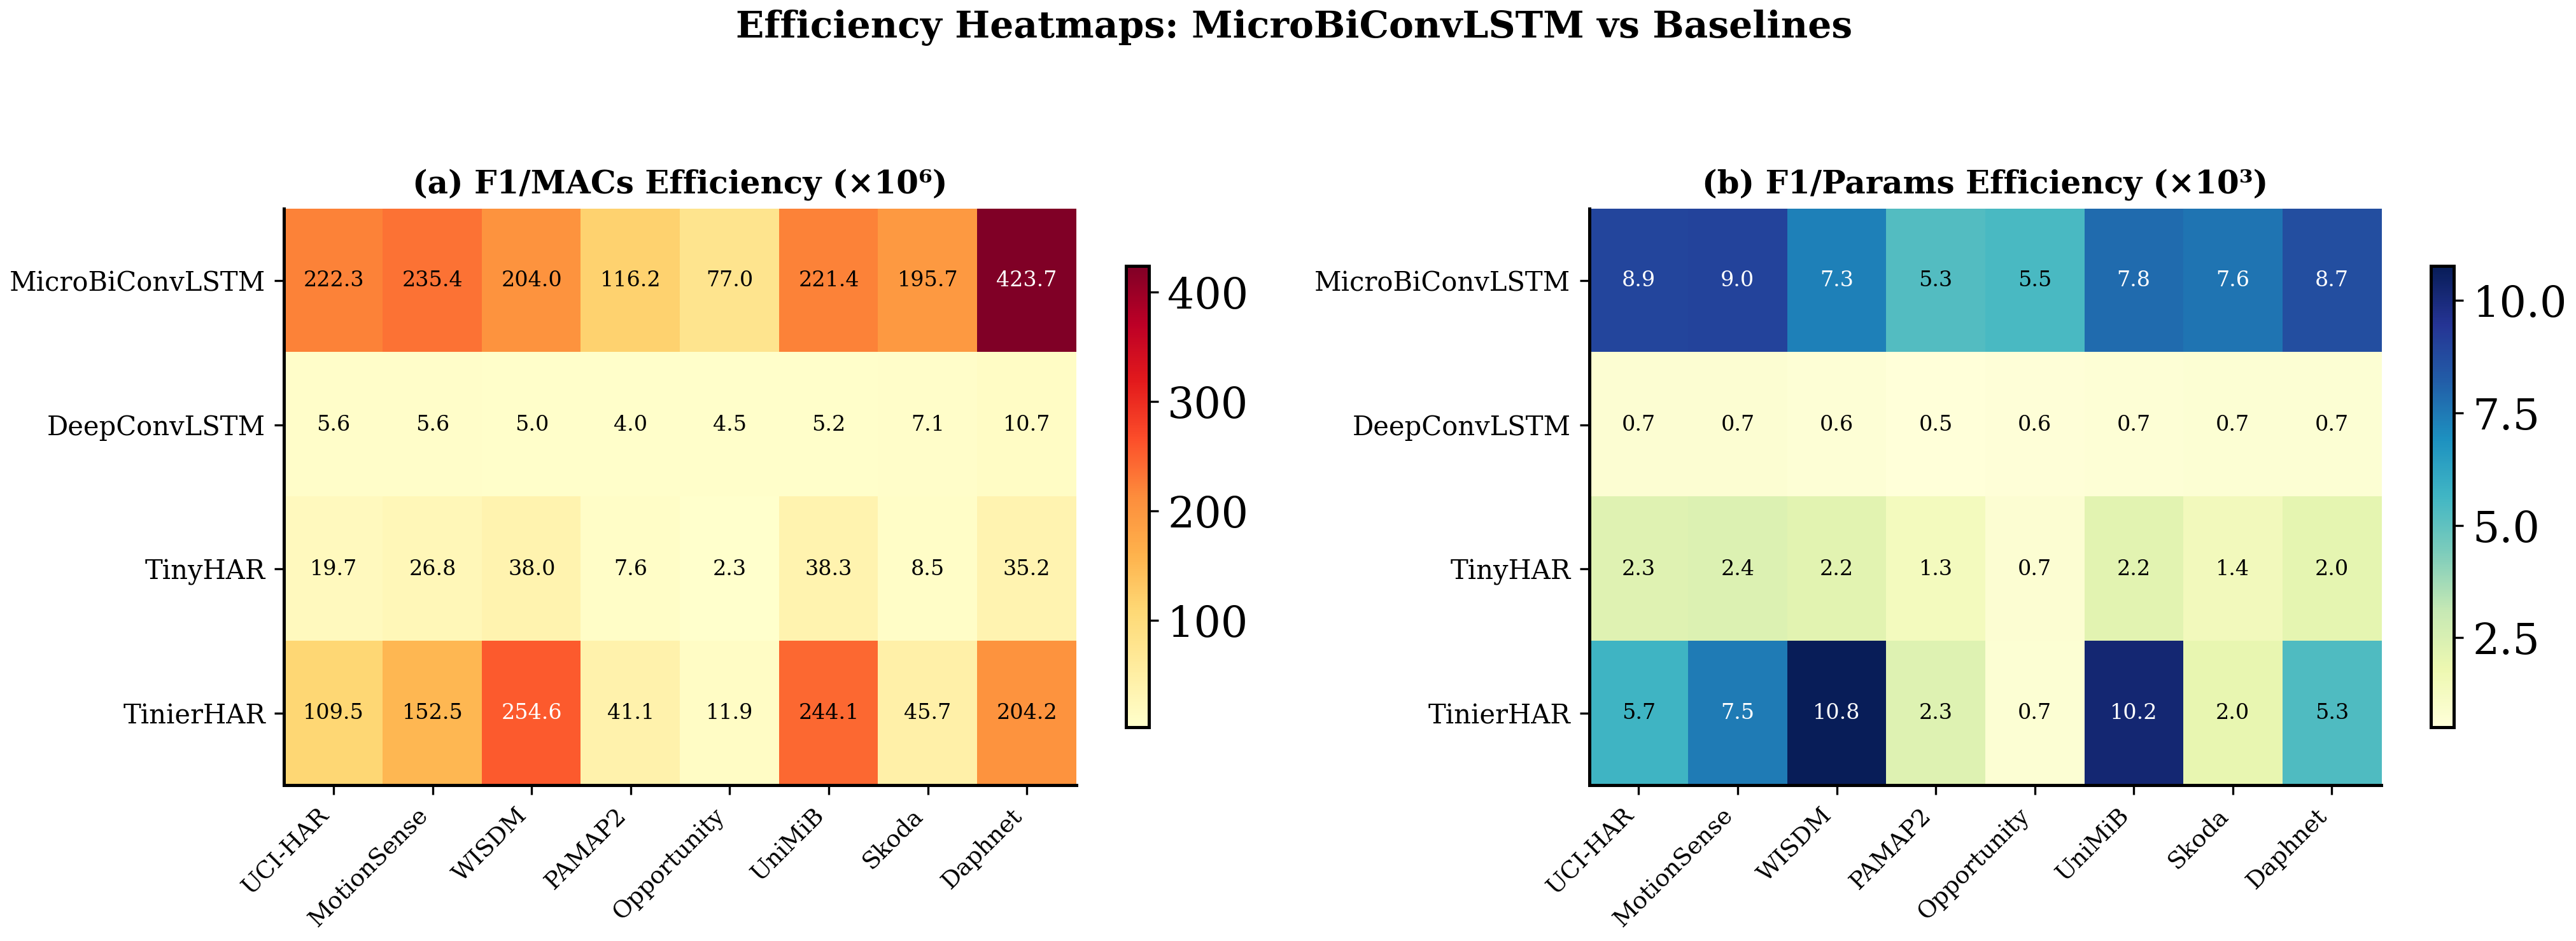
\includegraphics[width=\textwidth]{img/efficiency_heatmap.png}
        \caption{Efficiency heatmap}
    \end{subfigure}
    \caption{(a) Macro F1 against MACs on a log scale. (b) Macro F1 per million MACs and per thousand parameters.}
    \label{fig:efficiency_combined}
\end{figure}

Figure~\ref{fig:efficiency_combined} places \modelname{} in the high efficiency Pareto region. Table~\ref{tab:efficiency} reports 7.34 macro F1 points per thousand parameters. This is 2.8$\times$ the value of TinierHAR. The compact student already operates near the observed accuracy to parameter efficiency limit of its fixed design. Its small capacity may limit how closely it can match softened teacher outputs. This may explain the limited gains on most datasets. Teacher assistant distillation targets such capacity gaps \cite{mirzadeh2020improved}, yet it gives no consistent gain here.

\subsection{UCI-HAR Training Curves}

\begin{figure*}[!t]
    \centering
    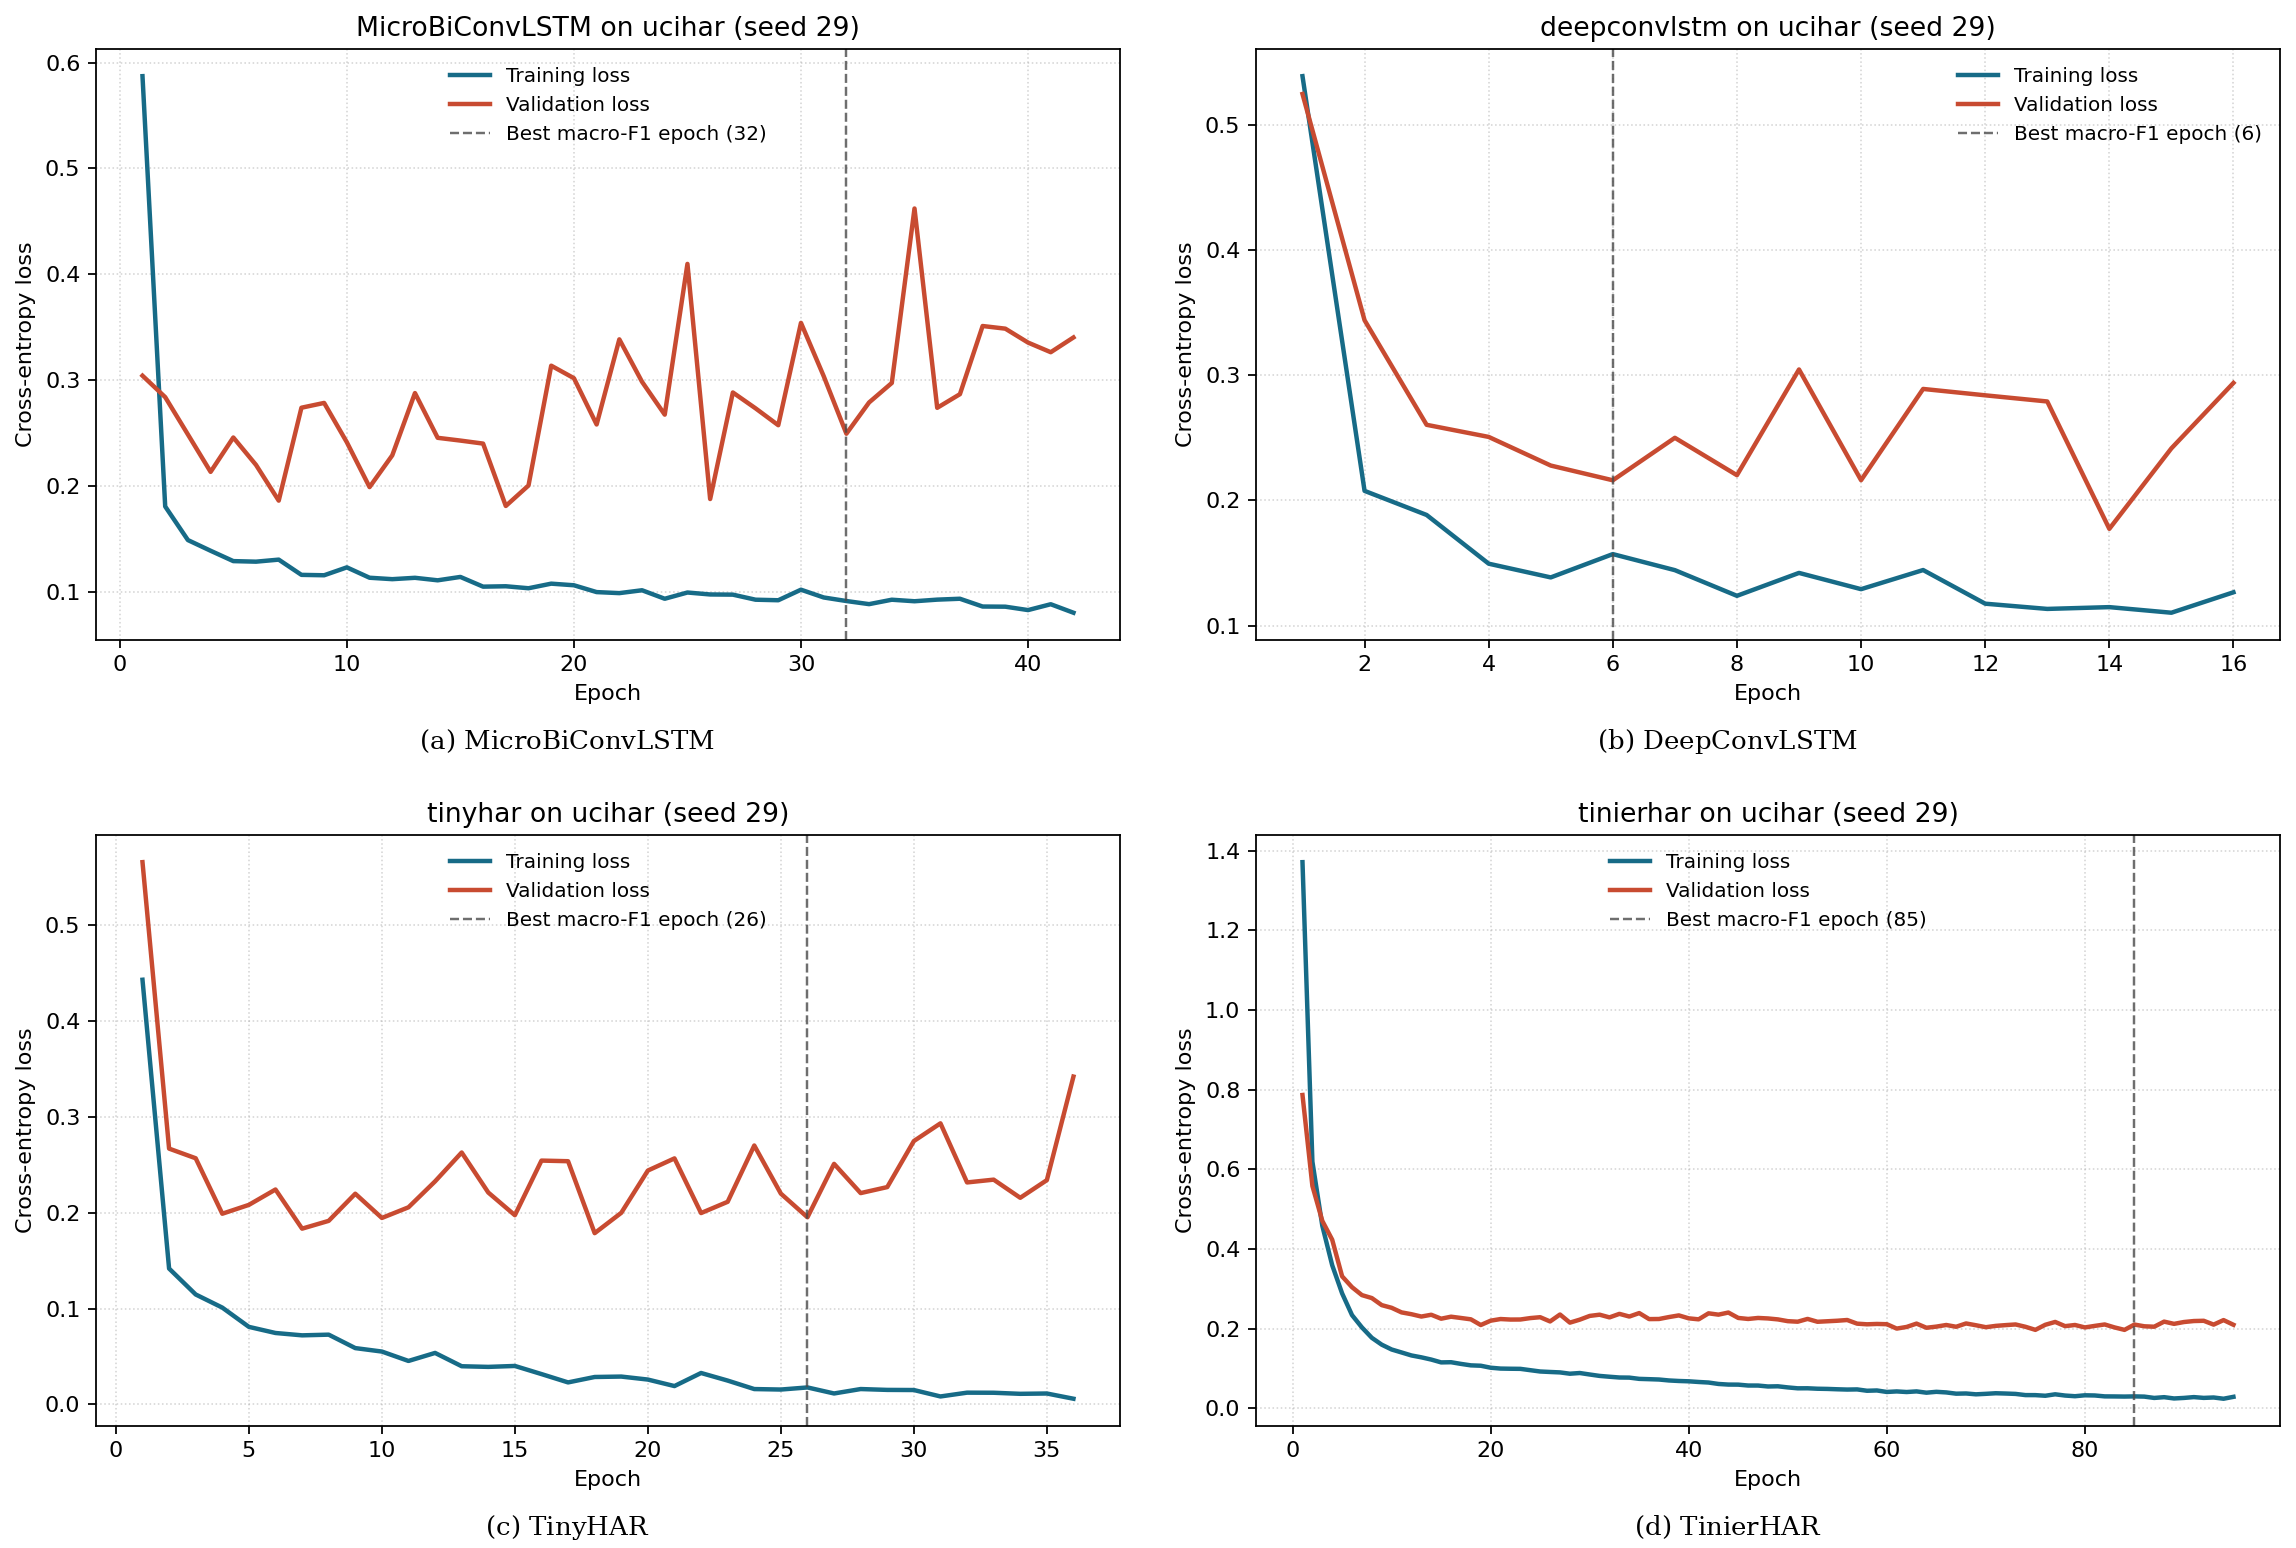
\includegraphics[width=0.82\textwidth]{img/ucihar_loss_curves_2x2.png}
    \caption{UCI-HAR loss histories for one random seed: (a) \modelnameplain{}, (b) DeepConvLSTM, (c) TinyHAR and (d) TinierHAR. Dashed lines mark the epoch with the highest recorded macro F1. Validation loss comes from the held out evaluation loader used by the trainers.}
    \label{fig:ucihar_curves}
\end{figure*}

\begin{figure*}[!b]
    \centering
    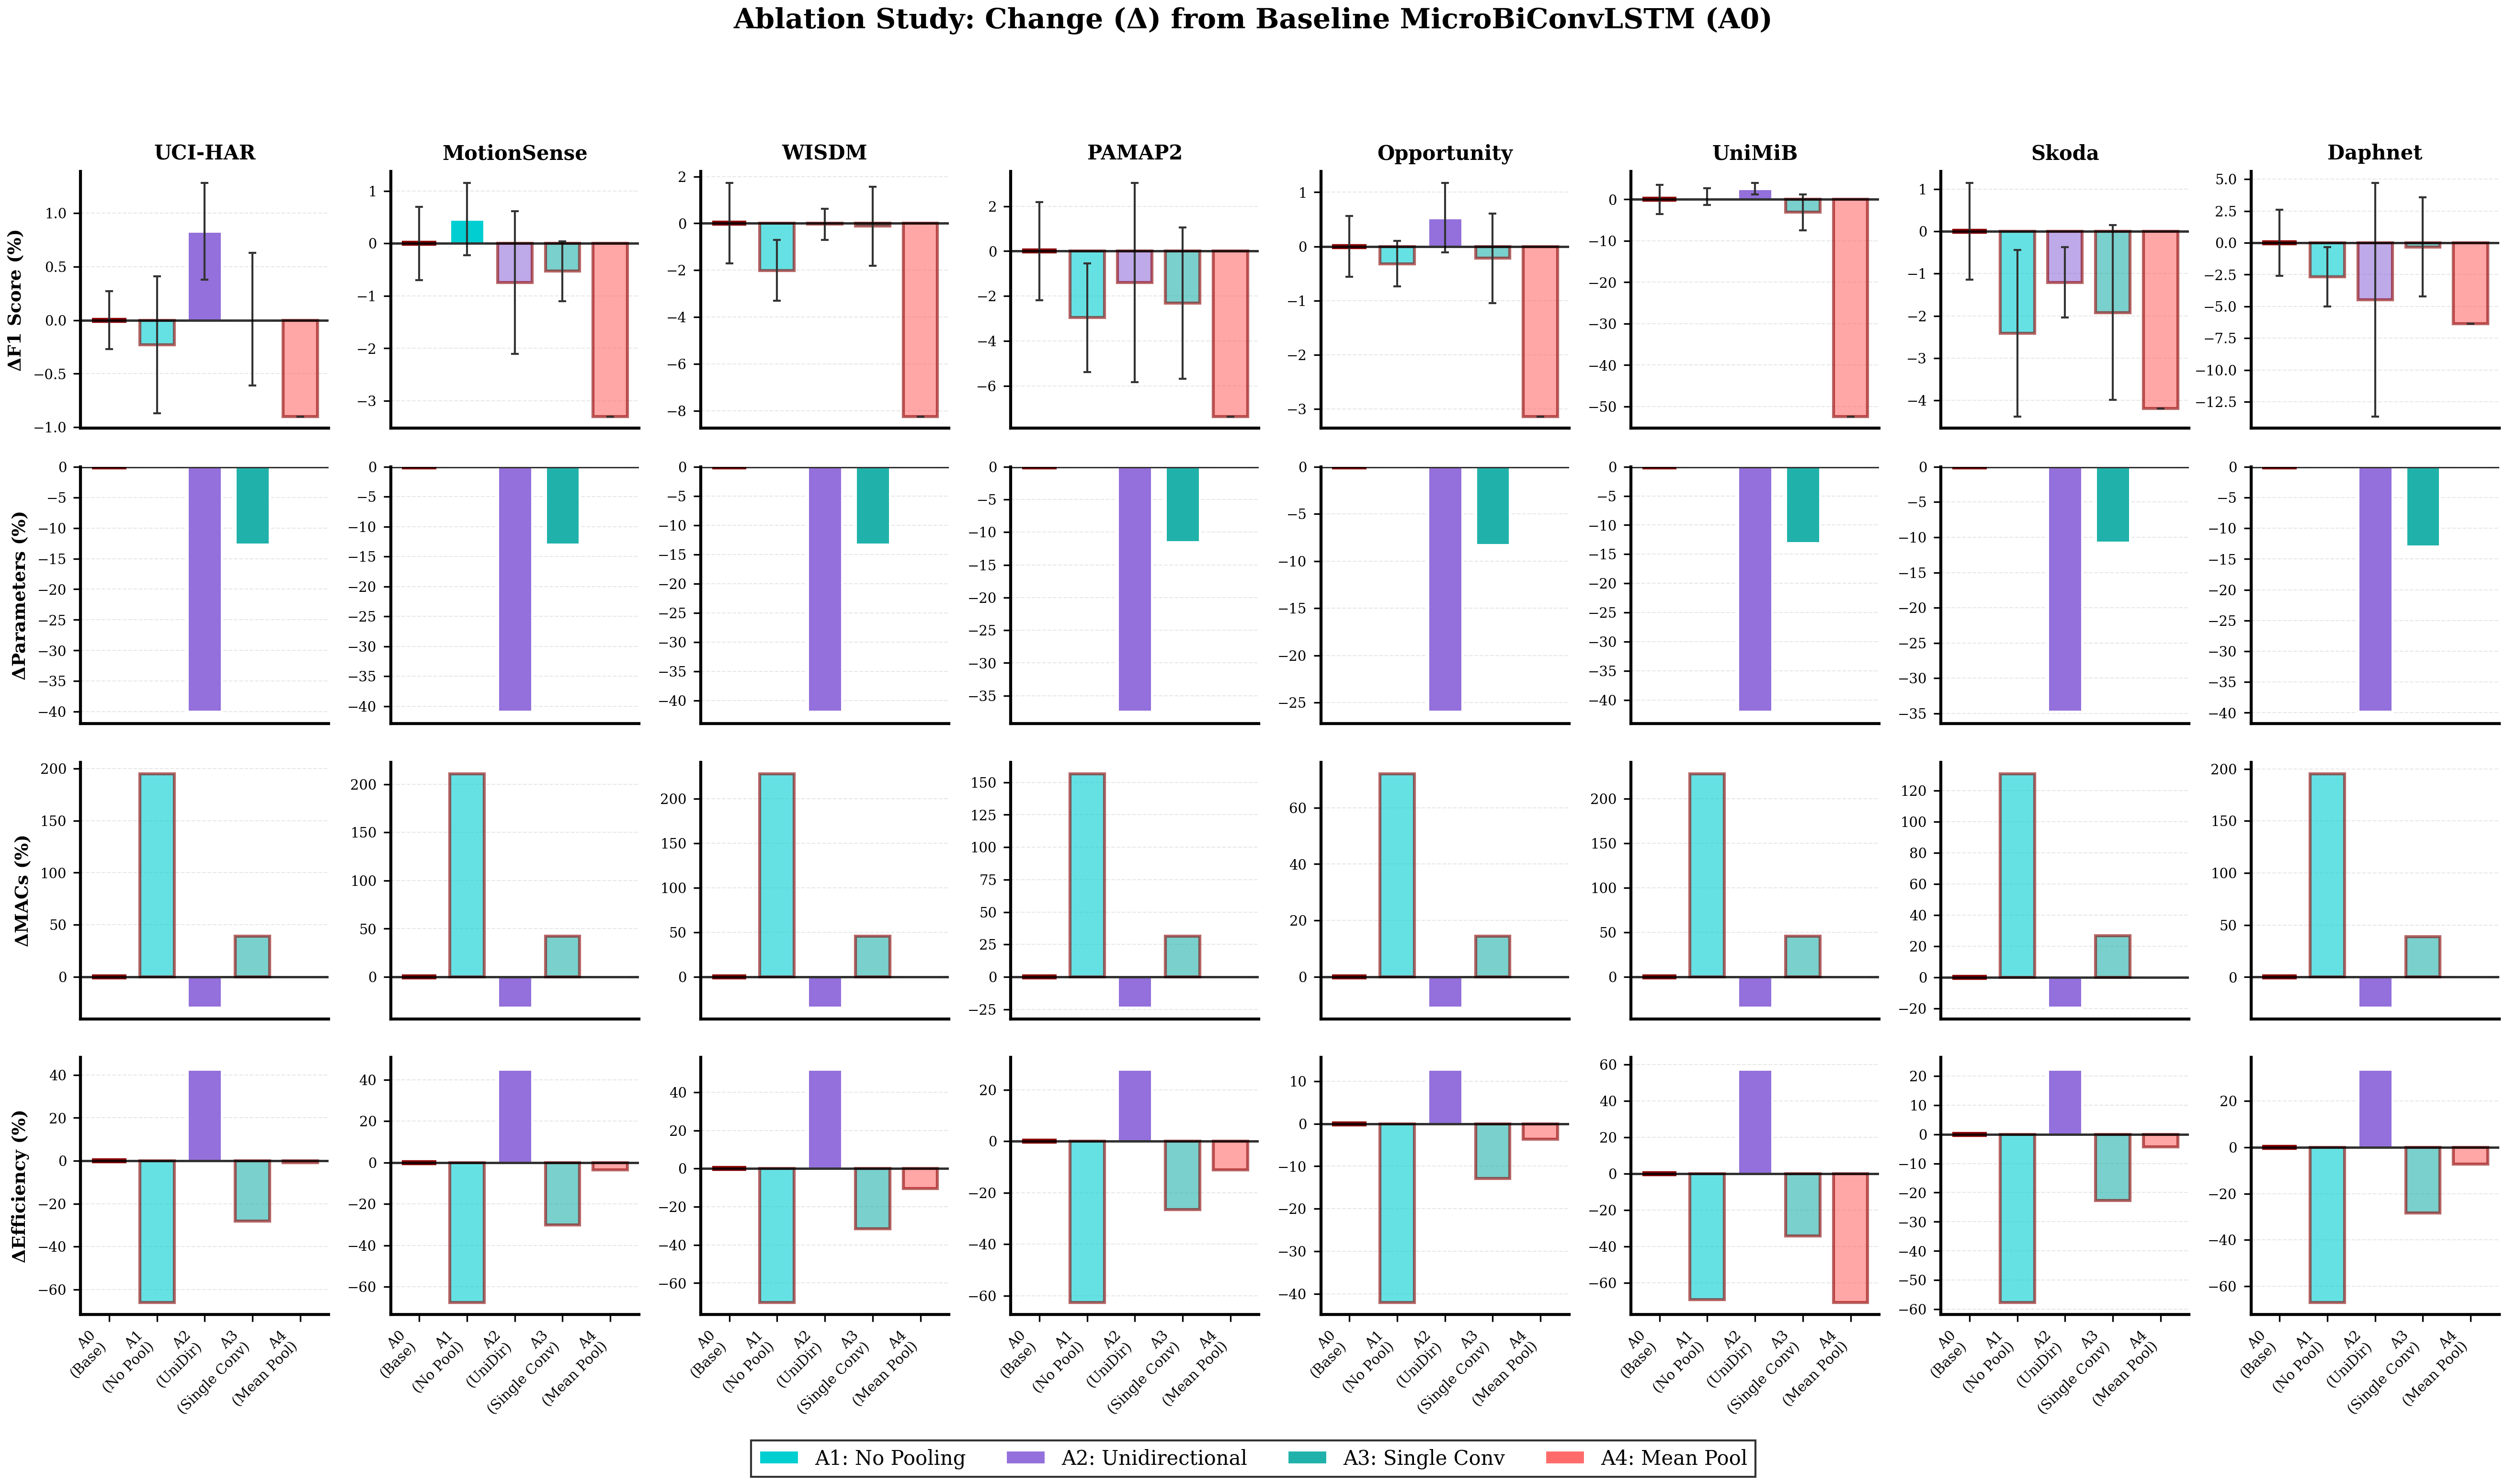
\includegraphics[width=0.64\textwidth]{img/ablation_study_grid.png}
    \caption{Ablation results across variants A0 to A4 and datasets. A0 is the base configuration. A1 removes pooling. A2 uses a unidirectional LSTM. A3 uses one convolutional block. A4 uses mean pooling.}
    \label{fig:ablation_grid}
\end{figure*}

Figure~\ref{fig:ucihar_curves} shows loss histories for the four neural models using one random seed. Training loss falls for every model. The held out curve is noisier for \modelname{}, DeepConvLSTM and TinyHAR. The implemented trainers evaluate the held out loader after every epoch and select the checkpoint with the highest macro F1. These curves document the implemented protocol. They do not use an independent validation split.

\subsection{Computational Efficiency}

\begin{table}[!t]
\centering
\caption{Computational Efficiency Comparison}
\label{tab:efficiency}
\resizebox{\columnwidth}{!}{%
\begin{tabular}{@{}lcccc@{}}
\toprule
\textbf{Metric} & \textbf{\modelnameplain{}} & \textbf{DeepConvLSTM} & \textbf{TinyHAR} & \textbf{TinierHAR} \\
\midrule
Parameters $\downarrow$ & \textbf{11.4K} & 135.6K & 55.1K & 33.5K \\
MACs $\downarrow$ & \textbf{485K} & 15.51M & 9.29M & 1.73M \\
F1/K-Params $\uparrow$ & \textbf{7.34} & 0.63 & 1.56 & 2.61 \\
F1/M-MACs $\uparrow$ & \textbf{172.5} & 5.54 & 9.27 & 50.5 \\
Complexity & $O(N)$ & $O(N)$ & $O(N^2)$ & $O(N^2)$ \\
\bottomrule
\end{tabular}%
}\vspace{1.5mm}
\end{table}

\begin{table}[!t]
\centering
\caption{MACs by Dataset (thousands)}
\label{tab:macs_per_dataset}
\resizebox{\columnwidth}{!}{%
\begin{tabular}{@{}lrrrr@{}}
\toprule
\textbf{Dataset} & \textbf{\modelnameplain{} $\downarrow$} & \textbf{DeepConvLSTM $\downarrow$} & \textbf{TinyHAR $\downarrow$} & \textbf{TinierHAR $\downarrow$} \\
\midrule
UCI-HAR & \textbf{420} & 16,620 & 6,050 & 1,080 \\
MotionSense & \textbf{389} & 16,490 & 4,270 & 740 \\
WISDM & \textbf{359} & 16,370 & 2,480 & 402 \\
PAMAP2 & \textbf{523} & 17,030 & 12,010 & 2,210 \\
Opportunity & \textbf{1,140} & 19,480 & 47,770 & 8,970 \\
UniMiB & \textbf{359} & 16,370 & 2,480 & 402 \\
SKODA & \textbf{444} & 13,290 & 12,360 & 1,910 \\
Daphnet & \textbf{245} & 8,110 & 2,640 & 399 \\
\midrule
\textbf{Average} & \textbf{485} & 15,510 & 9,290 & 1,730 \\
\bottomrule
\end{tabular}%
}
\end{table}

Table~\ref{tab:efficiency} reports efficiency. \modelname{} reaches 7.34 F1 per thousand parameters and 172.5 F1 per million MACs. These values are 2.8$\times$ and 3.4$\times$ higher than TinierHAR. Figure~\ref{fig:efficiency_combined} shows the Pareto region. Table~\ref{tab:macs_per_dataset} reports the MAC count for each model and dataset. On 79 channel Opportunity, \modelname{} needs 1.14M MACs compared with 47.8M for TinyHAR.

\FloatBarrier
\newpage

\section{Ablation Studies}\vspace{-1mm}
\label{sec:ablation}

Five variants test the architecture in Figure~\ref{fig:ablation_grid}. Removing the backward pass reduces Daphnet F1 by 4.48\% while increasing UCI-HAR F1 by 0.83\%. This difference shows that episodic events benefit more from bidirectional context. Mean pooling reduces UniMiB F1 by 52.43\% because it weakens short fall events. Removing temporal pooling raises MACs by 3.1$\times$ with mixed accuracy changes. Increasing the filter and hidden dimensions gives only 0.79\% more F1 while almost doubling the parameter count.

\section{Discussion}

The results show that strong compression can retain useful accuracy when the design matches the task. \modelname{} stays within 3\% of larger baselines on UCI-HAR and MotionSense. It also reaches 94.46\% on SKODA and 88.98\% on Daphnet. PAMAP2 remains difficult because rare activities form less than 10\% of its samples, though direct distillation improves the five seed mean by 2.71 points and improves every paired run. Direct distillation also gives smaller mean gains on UniMiB and SKODA. Other distillation comparisons are mixed. The ablation results show that bidirectionality is not equally useful for every activity type. Larger models remain preferable when accuracy matters more than parameter efficiency.

\section{Conclusion}

\modelname{} is a lightweight HAR architecture with 11.4K parameters on average. It uses 2.9$\times$ fewer parameters than TinierHAR while retaining competitive accuracy. Its main design choices are 4$\times$ temporal pooling, one bidirectional LSTM layer and last timestep aggregation.

Evaluation across eight datasets reveals both strengths and limits. \modelname{} performs well on smartphone IMU data and binary medical classification. Severe class imbalance reduces its macro F1 score. Bidirectionality helps episodic event detection while it gives limited or negative effects on periodic activities.

These findings show that models below 15K parameters can support single sensor wearable tasks. Careful matching between the task and architecture remains necessary. Future work will study sensor specific architecture search and distillation objectives designed for very small students.

\noindent\textbf{Code:} \url{https://github.com/WhiteMetagross/IMLProject}

\balance
\bibliographystyle{IEEEtran}
{\scriptsize
\begin{thebibliography}{14}

\bibitem{ordonez2016deep}
F.~J. Ord\'{o}\~{n}ez and D.~Roggen, ``Deep convolutional and LSTM recurrent neural networks for multimodal wearable activity recognition,'' \textit{Sensors}, vol.~16, no.~1, p.~115, 2016, doi: 10.3390/s16010115.

\bibitem{zhou2022tinyhar}
Y.~Zhou, H.~Zhao, Y.~Huang, M.~Hefenbrock, T.~Riedel and M.~Beigl, ``TinyHAR: A lightweight deep learning model designed for human activity recognition,'' in \textit{Proc. ACM Int. Symp. Wearable Comput.}, 2022, pp.~89--93, doi: 10.1145/3544794.3558467.

\bibitem{bian2025tinierhar}
S.~Bian, M.~Liu, V.~F.~Rey, D.~Geissler and P.~Lukowicz, ``TinierHAR: Towards ultra-lightweight deep learning models for efficient human activity recognition on edge devices,'' 2025.

\bibitem{chen2016xgboost}
T.~Chen and C.~Guestrin, ``XGBoost: A scalable tree boosting system,'' in \textit{Proc. 22nd ACM SIGKDD Int. Conf. Knowl. Discovery Data Mining}, 2016, pp.~785--794, doi: 10.1145/2939672.2939785.

\bibitem{kwapisz2011activity}
J.~R. Kwapisz, G.~M. Weiss and S.~A. Moore, ``Activity recognition using cell phone accelerometers,'' \textit{ACM SIGKDD Explor. Newsl.}, vol.~12, no.~2, pp.~74--82, 2010, doi: 10.1145/1964897.1964918.

\bibitem{anguita2013public}
D.~Anguita, A.~Ghio, L.~Oneto, X.~Parra and J.~L. Reyes-Ortiz, ``A public domain dataset for human activity recognition using smartphones,'' in \textit{Proc. Eur. Symp. Artif. Neural Netw.}, 2013, pp.~437--442.

\bibitem{malekzadeh2019mobile}
M.~Malekzadeh, R.~G. Clegg, A.~Cavallaro and H.~Haddadi, ``Mobile sensor data anonymization,'' in \textit{Proc. ACM/IEEE Int. Conf. Internet Things Design Implement.}, 2019, pp.~49--58, doi: 10.1145/3302505.3310068.

\bibitem{chavarriaga2013opportunity}
R.~Chavarriaga, H.~Sagha, A.~Calatroni, S.~T. Digumarti, G.~Tr\"{o}ster, J.~d.~R. Mill\'{a}n and D.~Roggen, ``The Opportunity challenge: A benchmark database for on-body sensor-based activity recognition,'' \textit{Pattern Recognit. Lett.}, vol.~34, no.~15, pp.~2033--2042, 2013, doi: 10.1016/j.patrec.2012.12.014.

\bibitem{stiefmeier2008wearable}
T.~Stiefmeier, D.~Roggen, G.~Ogris, P.~Lukowicz and G.~Tr\"{o}ster, ``Wearable activity tracking in car manufacturing,'' \textit{IEEE Pervasive Comput.}, vol.~7, no.~2, pp.~42--50, 2008, doi: 10.1109/MPRV.2008.40.

\bibitem{bachlin2010wearable}
M.~B\"{a}chlin, M.~Plotnik, D.~Roggen, I.~Maidan, J.~M. Hausdorff, N.~Giladi and G.~Tr\"{o}ster, ``Wearable assistant for Parkinson's disease patients with the freezing of gait symptom,'' \textit{IEEE Trans. Inf. Technol. Biomed.}, vol.~14, no.~2, pp.~436--446, 2010, doi: 10.1109/TITB.2009.2036165.

\bibitem{reiss2012introducing}
A.~Reiss and D.~Stricker, ``Introducing a new benchmarked dataset for activity monitoring,'' in \textit{Proc. Int. Symp. Wearable Comput.}, 2012, pp.~108--109, doi: 10.1109/ISWC.2012.13.

\bibitem{micucci2017unimib}
D.~Micucci, M.~Mobilio and P.~Napoletano, ``UniMiB SHAR: A dataset for human activity recognition using acceleration data from smartphones,'' \textit{Appl. Sci.}, vol.~7, no.~10, p.~1101, 2017, doi: 10.3390/app7101101.

\bibitem{hinton2015distilling}
G.~Hinton, O.~Vinyals and J.~Dean, ``Distilling the knowledge in a neural network,'' in \textit{Proc. NIPS Deep Learning and Representation Learning Workshop}, 2015.

\bibitem{mirzadeh2020improved}
S.~I. Mirzadeh, M.~Farajtabar, A.~Li, N.~Levine, A.~Matsukawa and H.~Ghasemzadeh, ``Improved knowledge distillation via teacher assistant,'' in \textit{Proc. AAAI Conf. Artif. Intell.}, vol.~34, no.~4, pp.~5191--5198, 2020, doi: 10.1609/aaai.v34i04.5963.

\end{thebibliography}
}

\end{document}
